\usetikzlibrary{babel}
\begin{figure}[htb]
\centering
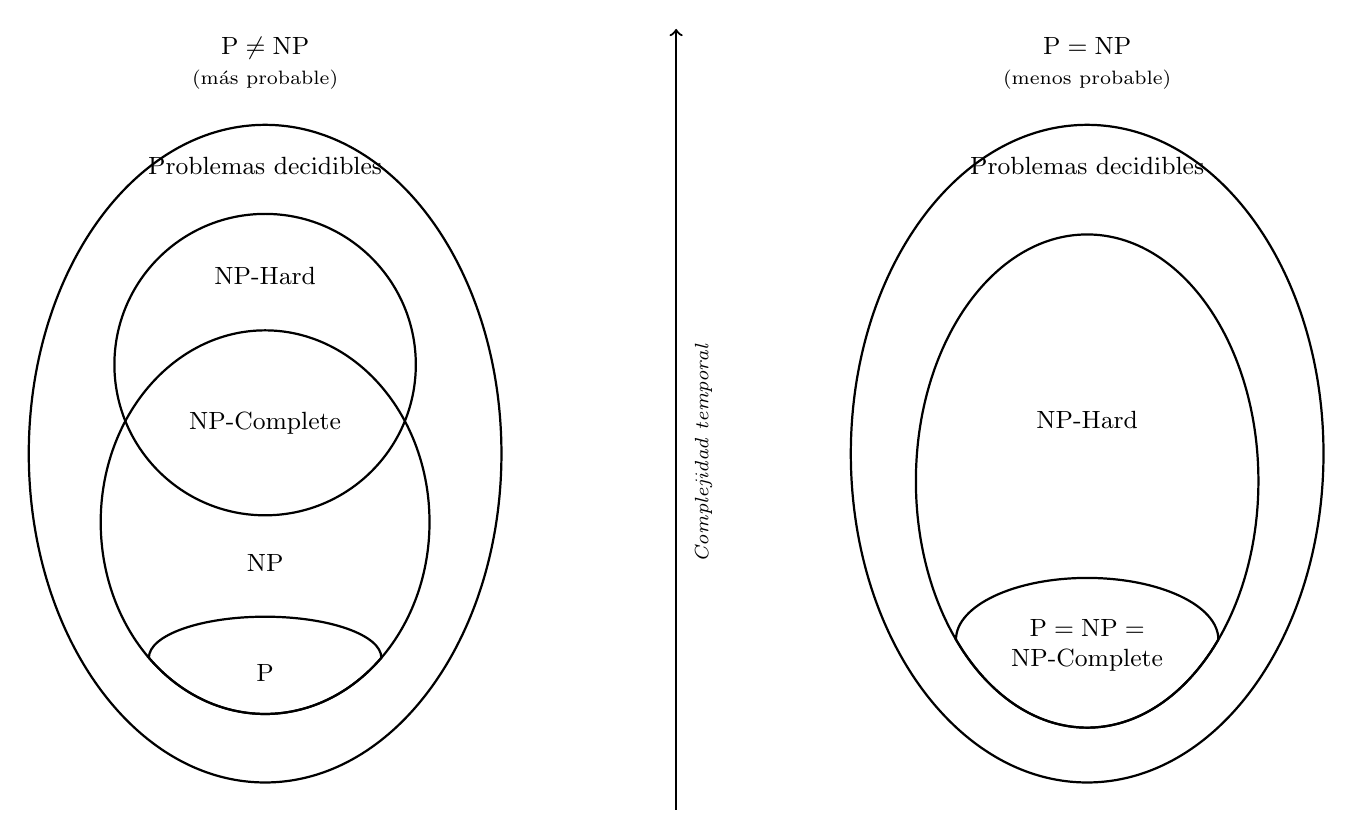
\begin{tikzpicture}[scale=0.87, font=\small, thick]

  %% =================== VERTICAL AXIS ====================
  \draw[->] (0, -5.2) -- (0, 6.2);
  \node[rotate=90, font=\itshape\scriptsize] at (0.4, 0) {Complejidad temporal};

  %% ================= LEFT PANEL: P ≠ NP =================

  \node[align=center] at (-6, 5.7)
    {$\mathrm{P} \neq \mathrm{NP}$ \\ {\scriptsize (más probable)}};

  % Outer oval: Problemas decidibles
  \draw (-6, 0) ellipse (3.45 and 4.8);
  \node at (-6, 4.2) {Problemas decidibles};

  % NP oval (lower)
  \draw (-6, -1.0) ellipse (2.4 and 2.8);
  \node at (-6, -1.6) {NP};

  % NP-Hard oval (upper, overlapping NP)
  \draw (-6, 1.3) ellipse (2.2 and 2.2);
  \node at (-6, 2.6) {NP-Hard};

  % NP-Complete label: inside NP ∩ NP-Hard
  \node at (-6, 0.45) {NP-Complete};

  % P shape: bottom arc follows NP oval, closed with a dome.
  % Junctions at 225°/315° of NP oval: (−7.697, −2.980) and (−4.303, −2.980).
  \draw (-7.697, -2.980)
    arc[start angle=225, end angle=315, x radius=2.4, y radius=2.8]
    arc[start angle=0, end angle=180, x radius=1.697, y radius=0.6]
    -- cycle;
  \node at (-6, -3.2) {P};

  %% ================ RIGHT PANEL: P = NP ================

  \node[align=center] at (6, 5.7)
    {$\mathrm{P} = \mathrm{NP}$ \\ {\scriptsize (menos probable)}};

  % Outer oval: Problemas decidibles
  \draw (6, 0) ellipse (3.45 and 4.8);
  \node at (6, 4.2) {Problemas decidibles};

  % NP-Hard oval
  \draw (6, -0.4) ellipse (2.5 and 3.6);
  \node at (6, 0.5) {NP-Hard};

  % P=NP=NP-Complete shape: bottom arc follows NP-Hard oval, closed with a dome.
  % Junctions at 220°/320° of NP-Hard oval: (4.085, −2.714) and (7.915, −2.714).
  \draw (4.085, -2.714)
    arc[start angle=220, end angle=320, x radius=2.5, y radius=3.6]
    arc[start angle=0, end angle=180, x radius=1.915, y radius=0.9]
    -- cycle;
  \node[align=center] at (6, -2.8)
    {$\mathrm{P} = \mathrm{NP} =$\\NP-Complete};

\end{tikzpicture}
\caption{Clasificación de los problemas computables por clases de complejidad, para los dos escenarios del problema abierto $\mathrm{P}$ vs.\ $\mathrm{NP}$.}
\label{fig:p-vs-np}
\end{figure}
